\documentclass[10pt]{article}
\usepackage[margin=0.72in]{geometry}
\usepackage{booktabs}
\usepackage{tikz}
\usepackage[T1]{fontenc}
\begin{document}
\section*{p739 retained cross-session audit}
\textbf{Observations only.} This report records a native, solver-free comparison of two preserved sessions. It makes no timing, ratio, admission, or scientific-priority judgment.

\subsection*{Recorded comparison}
\begin{tabular}{lr}
\toprule
Quantity & Count \\
\midrule
Records in each session & 1080 \\
Exact deterministic solver/accounting projections & 1080 \\
Measured rows replayed identically by each retained audit & 900 \\
Warmups statically verified and cross-session compared & 180 \\
Disallowed differing paths & 0 \\
New solver executions / measurements & 0 / 0 \\
\bottomrule
\end{tabular}

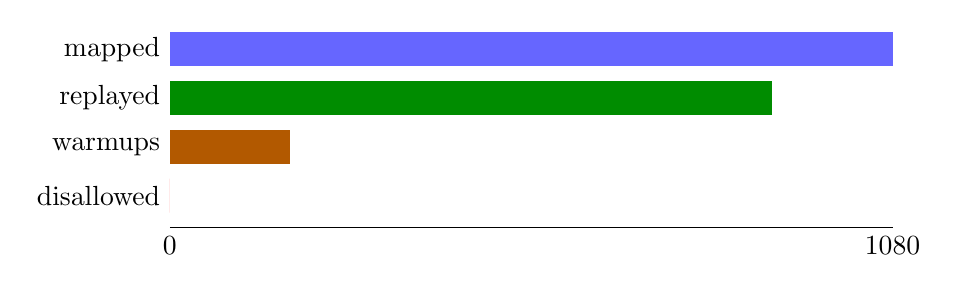
\begin{tikzpicture}[x=0.0085cm,y=0.62cm]
\node[anchor=east] at (0,0) {mapped}; \fill[blue!60] (0,-0.35) rectangle (1080,0.35);
\node[anchor=east] at (0,-1) {replayed}; \fill[green!55!black] (0,-1.35) rectangle (900,-0.65);
\node[anchor=east] at (0,-2) {warmups}; \fill[orange!70!black] (0,-2.35) rectangle (180,-1.65);
\node[anchor=east] at (0,-3) {disallowed}; \fill[red!65] (0,-3.35) rectangle (0,-2.65);
\draw (0,-3.65) -- (1080,-3.65); \node[anchor=north] at (0,-3.65) {0}; \node[anchor=north] at (1080,-3.65) {1080};
\end{tikzpicture}

\subsection*{Hash-bound result}
Normalized plan SHA-256: \texttt{\footnotesize 6627fb44589dacd3d79b8d28fdf0fb0df523cb53e3258b9713519a22439ff932}\\
Normalized specification SHA-256: \texttt{\footnotesize 523a99e19373bd205acd954bab9549e7fbe59830fd7273658f2b8f01eede3b8a}\\
Deterministic projection SHA-256: \texttt{\footnotesize 91338d7abcda1144d949d64d827de81d874ca49d07a2b536cd803f42ff78a3e1}\\
Projection bytes: 12286741.

The row mapping and complete input bindings are in \texttt{row-mapping.json} and \texttt{audit.json}. The comparison pairs exact unsigned 64-bit seeds; it never converts them to floating point. Every observed difference is checked against a fixed leaf-level allowlist before the deterministic solver/accounting projection is formed. An unlisted or newly differing field causes failure. The projection excludes wall and CPU timing, maximum RSS, faults, context switches, scheduler CPU observations, IRQ observations, isolation/environment fields, and session/record identities. It therefore does not establish equality of all non-wall or all resource content.

\subsection*{Fresh audit-receipt provenance}
The compared fresh audit is the exact retained bytes of one named, versioned remote result object. Its own timestamp is after session completion, its binary and environment identifiers match the fresh session, and the downloaded SHA manifest binds the same bytes. These records do not establish a separate auditor principal or process.

\subsection*{Review limits}
\begin{itemize}
\item Both sessions used the same measurement binary; this is not an independent implementation check.
\item The 900 measured rows were replayed identically by each retained ecbench audit receipt; 180 warmups were statically verified and cross-session compared but were not replay candidates.
\item Timing, isolation, environment, session IDs and record IDs are excluded; this does not validate wall time, admit ratios or qualify either session for a timing claim.
\item Excluded process-resource observations include maximum RSS, faults, voluntary and involuntary context switches, scheduler CPU time/CPU identity, IRQ observations, and user/system CPU time. No equality of complete resource costs is claimed.
\item The fresh receipt is version-bound and post-session, but the preserved evidence does not establish an independent auditor principal or process.
\item This software audit changes no frozen protocol, record, plan or measurement artifact.
\end{itemize}
\end{document}
